\documentclass[12pt,a4paper]{article}
\usepackage[utf8]{inputenc}
\usepackage{graphicx}
\usepackage{hyperref}
\usepackage{listings}
\usepackage{xcolor}
\usepackage{amsmath}
\usepackage{amssymb}
\usepackage{tabularx}
\usepackage{float}
\usepackage{geometry}
\usepackage{subcaption}
\usepackage{booktabs}
\usepackage{titling}
\geometry{margin=1in}
\hypersetup{
	colorlinks=true,
	linkcolor=blue,
	filecolor=magenta,
	urlcolor=cyan,
}
\title{Autonomous Robot with Traffic Light Detection System}
\author{}
\date{}
\begin{document}
	% Title Page
	\begin{titlepage}
		\centering
		\vspace*{2cm}
		{\Huge\bfseries Autonomous Robot with Traffic Light Detection System\par}
		\vspace{2cm}
		{\Large Robotics Project Report\par}
		\vspace{2cm}
		
		{\Large \textbf{Authors:}\par}
		\vspace{0.5cm}
		{\Large Moktar Sellami\par}
		{\Large Achref Fradj\par}
		{\Large Othmen Ben Ismail\par}
		\vspace{2cm}
		
		{\Large \textbf{Supervisor:}\par}
		\vspace{0.5cm}
		{\Large Sarra Ben Hlima\par}
		\vspace{2cm}
		
		{\Large \textbf{Class:}\par}
		\vspace{0.5cm}
		{\Large 3ISEOC\par}
		\vspace{2cm}
		
		{\Large \today\par}
	\end{titlepage}
	
	\tableofcontents
	\newpage
	
	\section{Project Overview}
	This project implements an autonomous robot capable of detecting and responding to traffic lights. The system combines embedded bare-metal programming on STM32 microcontroller with ROS2-based computer vision on Raspberry Pi, creating a complete autonomous navigation solution.
	\begin{figure}[H]
		\centering
		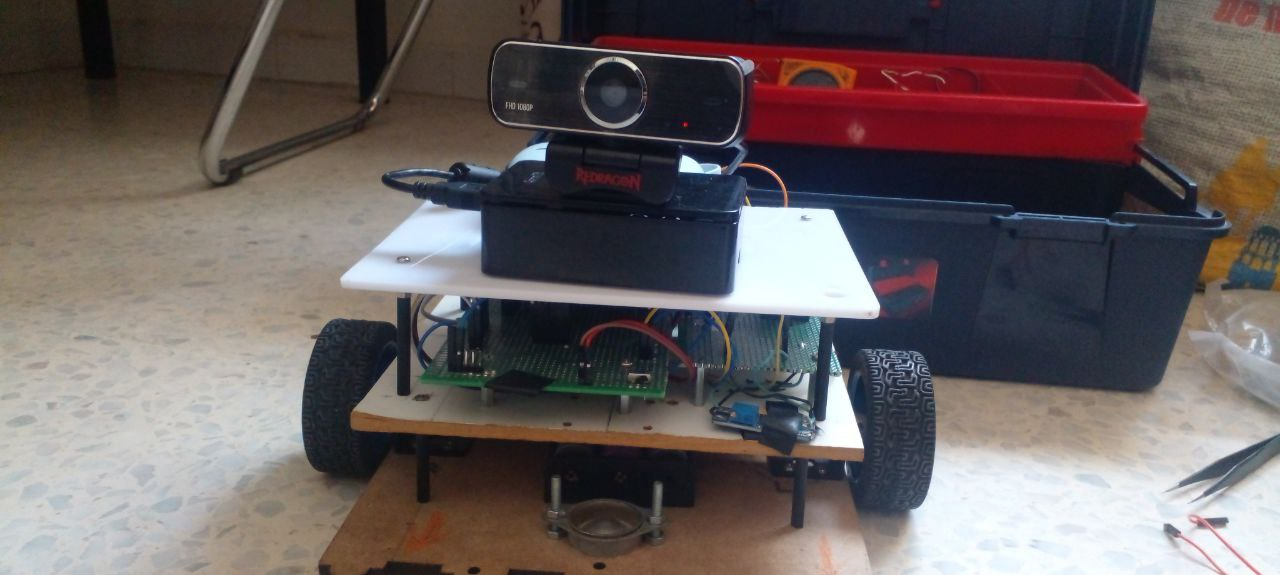
\includegraphics[width=0.8\textwidth]{robot.jpg}
		\caption{DagDeg Autonomous Robot}
		\label{fig:robot}
	\end{figure}
	
	\section{System Architecture}
	
	\begin{figure}[H]
		\centering
		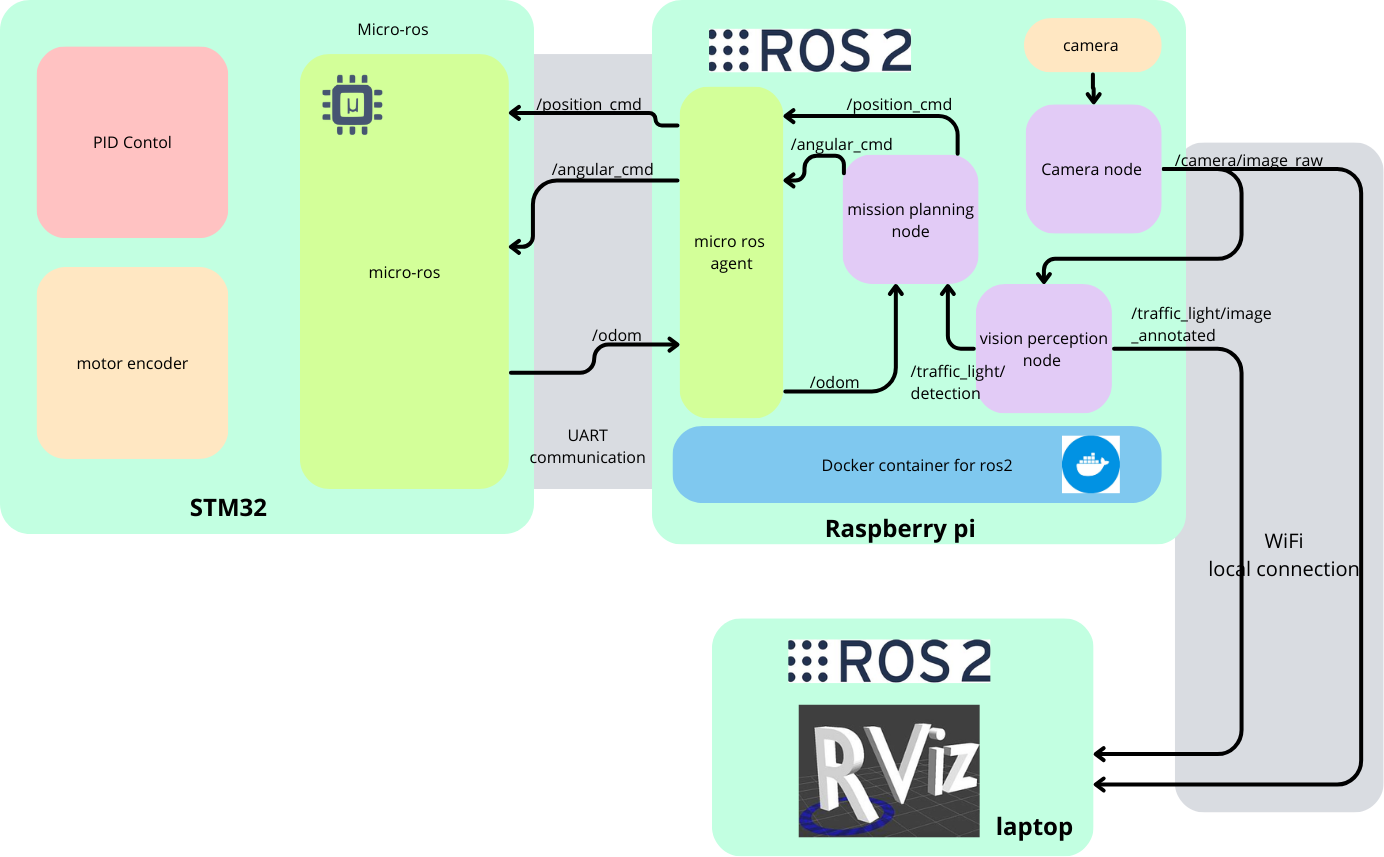
\includegraphics[width=0.8\textwidth]{system_arch.png}
		\caption{System Architecture Diagram}
		\label{fig:architecture}
	\end{figure}
	
	The system consists of three main components:
	\begin{itemize}
		\item \textbf{STM32 Microcontroller}: Handles low-level motor control, PID controllers, and odometry
		\item \textbf{Raspberry Pi}: Runs ROS2 in Docker container with computer vision pipeline
		\item \textbf{Laptop}: For visualization using RViz and system monitoring via local network
	\end{itemize}
	
	\section{Hardware Implementation}
	\begin{figure}[H]
		\centering
		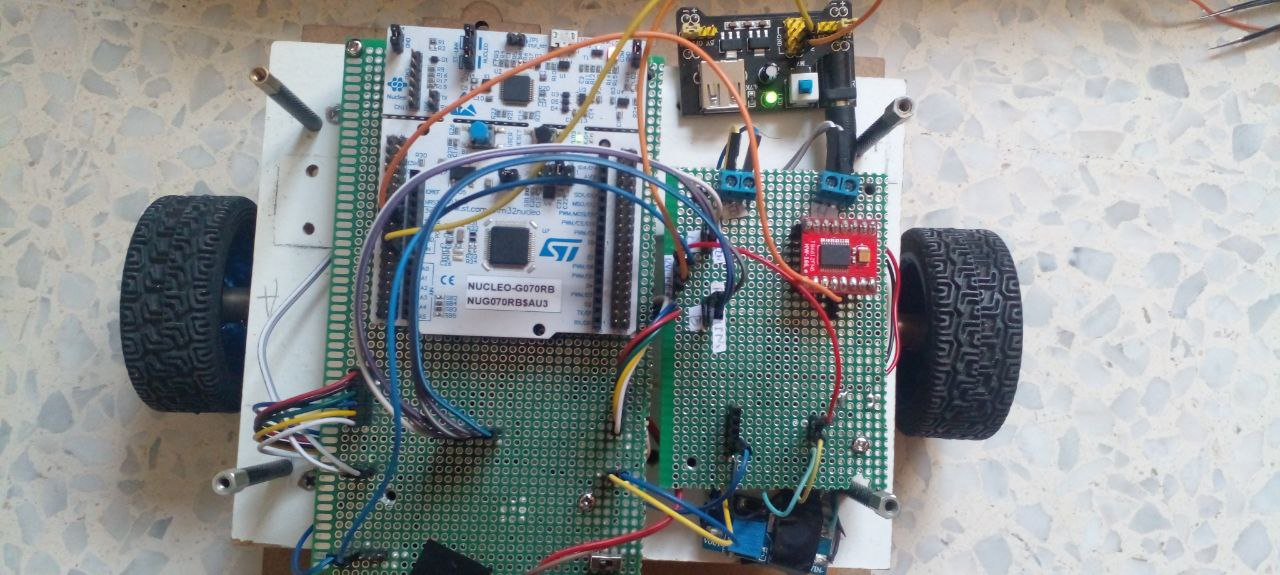
\includegraphics[width=0.8\textwidth]{hardware.jpg}
		\caption{Hardware Overview}
		\label{fig:Hardware}
	\end{figure}
	\subsection{Robot Fabrication}
	\begin{itemize}
		\item Custom chassis design and assembly
		\item Motor and wheel integration
		\item Power distribution system
		\item Camera mounting and positioning
		\item STM32 microcontroller integration
	\end{itemize}
	
	\section{STM32 Bare-Metal Development}
	
	The low-level firmware was developed using a bare-metal approach to achieve maximum timing precision. While this allowed for highly efficient PID loops, it presented a significant challenge for ROS2 integration. The lack of an abstraction layer and an RTOS meant that \texttt{micro-ROS}—which requires specific DMA and task-scheduling capabilities—could not be utilized. Instead, a custom communication protocol was developed.
	
	\subsection{Developed Drivers}
	\begin{table}[H]
		\centering
		\begin{tabularx}{\textwidth}{|l|X|}
			\hline
			\textbf{Driver} & \textbf{Description} \\
			\hline
			Motor Encoders & Quadrature encoder interface for position tracking \\
			UART Communication & Serial communication with Raspberry Pi \\
			Clock/System Configuration & Low-level system initialization \\
			PWM Motor Control & Precise motor speed control \\
			\hline
		\end{tabularx}
		\caption{STM32 Bare-Metal Drivers}
	\end{table}
	
	\subsection{PID Control System}
	
	\subsubsection{Position PID Controller}
	The robot utilizes a \textbf{dual-cascaded PID architecture}, featuring separate loops for position and angular control:
	\begin{itemize}
		\item \textbf{Position Control Cascade}: The outer loop controls the absolute target position (distance), while the inner loop regulates the linear velocity to ensure smooth movement.
		\item \textbf{Angular Control Cascade}: Similar to position control, this manages the robot's orientation, where the outer loop maintains the heading angle and the inner loop regulates angular velocity to minimize oscillations during turns.
	\end{itemize}
	
	\subsection{Odometry Module}
	\begin{itemize}
		\item Velocity measurement (linear and angular)
		\item Position tracking (x, y coordinates)
		\item Angle calculation (radians and degrees)
		\item Distance traveled computation
	\end{itemize}
	
	\subsection{Velocity Ramping System}
	
	A critical aspect of motion control is the implementation of velocity ramping for both linear and angular velocities. This system ensures smooth acceleration and deceleration, which is essential for several reasons:
	
	\begin{itemize}
		\item \textbf{Prevents Wheel Slipping}: Sudden acceleration changes can cause wheels to lose traction, especially on smooth surfaces
		\item \textbf{Reduces Mechanical Stress}: Gradual velocity changes minimize stress on motors, gears, and mechanical components
		\item \textbf{Improves Energy Efficiency}: Smooth acceleration profiles consume less power than jerky movements
		\item \textbf{Enhances System Stability}: Prevents overshoot and oscillations in the control system
		\item \textbf{Increases Position Accuracy}: Smooth velocity transitions lead to more precise position control
	\end{itemize}
	
	The ramping system was implemented for both linear velocity (\texttt{odo.v}) and angular velocity (\texttt{odo.w}) using a two-stage approach:
	
	1. \textbf{Ramp-Limited Setpoint}: A gradually increasing maximum velocity limit that prevents sudden jumps
	
	2. \textbf{Target Capping}: Ensures the commanded velocity never exceeds physical or safety limits
	
	\begin{figure}[H]
		\centering
		\begin{subfigure}{0.45\textwidth}
			\centering
			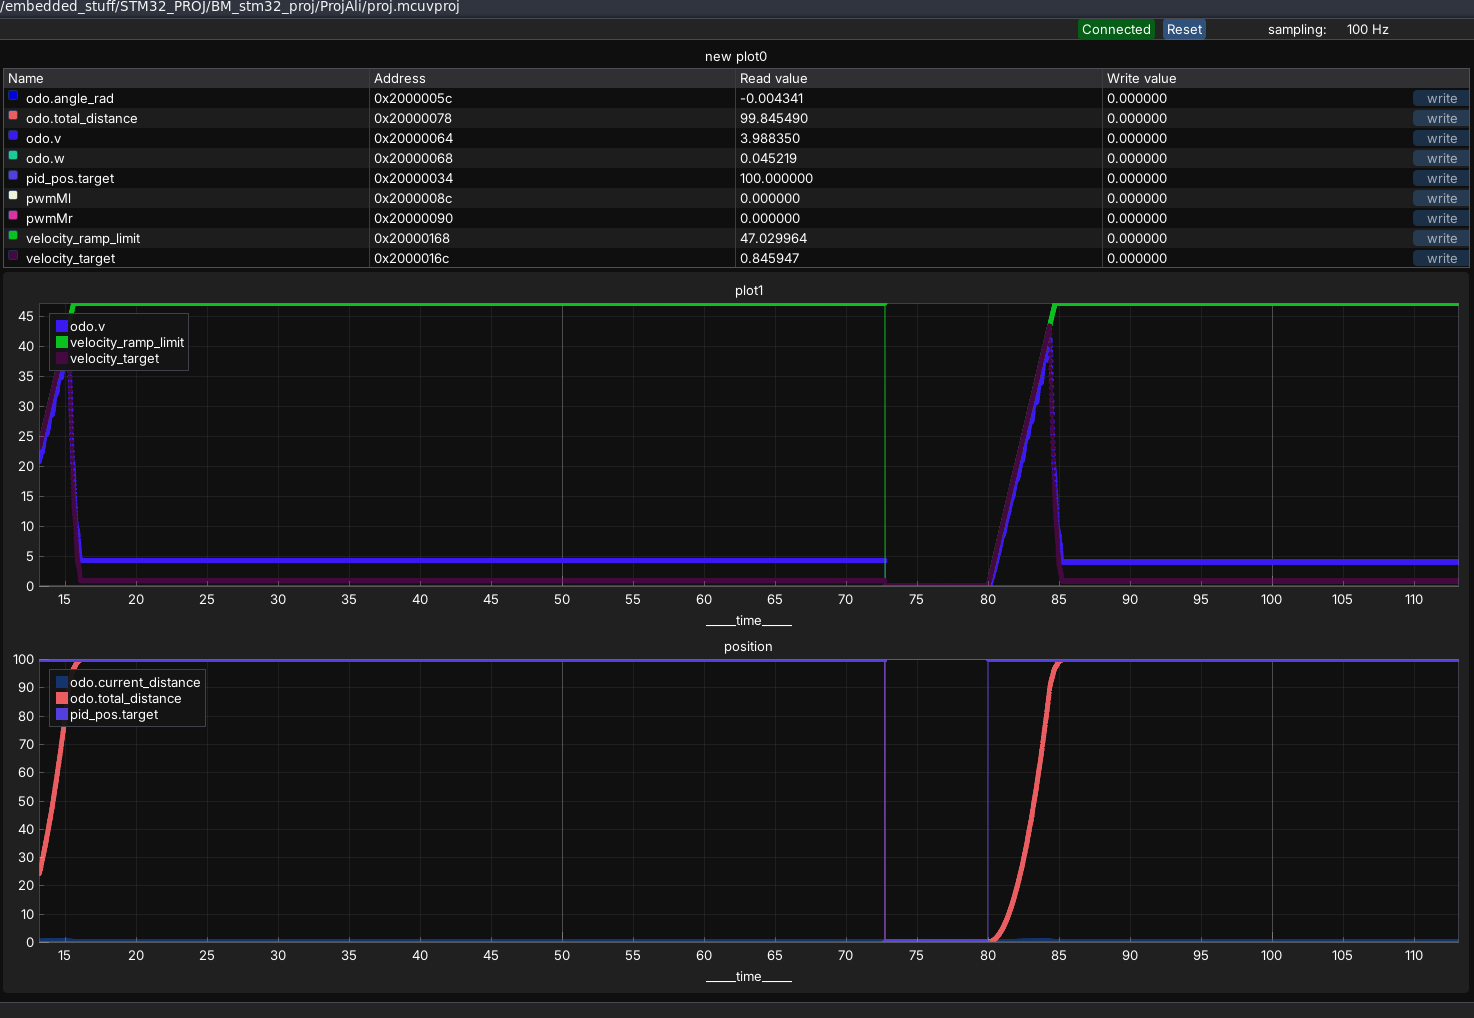
\includegraphics[width=\textwidth]{pid_pos_100.png}
			\caption{Linear Velocity Ramping Performance}
			\label{fig:linear_ramp}
		\end{subfigure}
		\begin{subfigure}{0.45\textwidth}
			\centering
			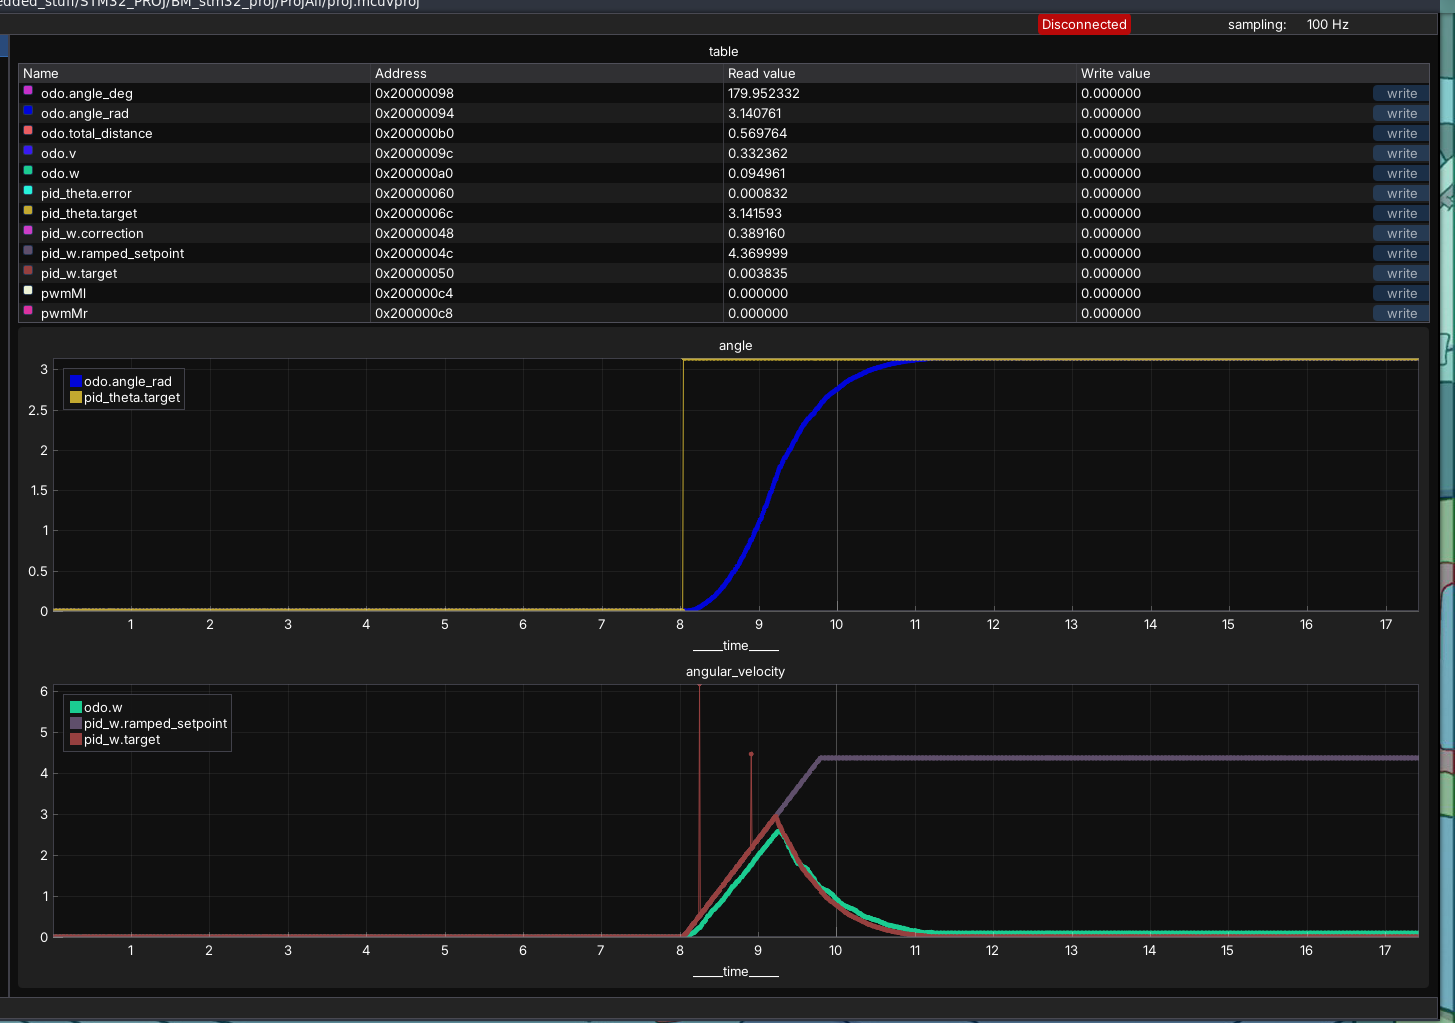
\includegraphics[width=\textwidth]{best_angle_control.png}
			\caption{Angular Velocity Ramping Performance}
			\label{fig:angular_ramp}
		\end{subfigure}
		\caption{Velocity Ramping System Performance}
		\label{fig:ramping_performance}
	\end{figure}
	
	As shown in Figure \ref{fig:ramping_performance}, the ramping system successfully achieves:
	\begin{itemize}
		\item Smooth acceleration from rest to target velocity
		\item Controlled deceleration when approaching target positions
		\item Elimination of velocity spikes that could destabilize the system
		\item Consistent performance across both linear and angular motion
	\end{itemize}
	
	\section{Traffic Light Detection Model}
	
	\subsection{Model Development Process}
	
	The traffic light detection model was developed using Google Colab, leveraging the following workflow:
	
	\begin{itemize}
		\item \textbf{Platform}: Google Colab with GPU acceleration
		\item \textbf{Notebook}: Available at \url{https://colab.research.google.com/drive/1lxwcOyEtk-aGk_w2Za_TbaYP-JJjzC9H}
		\item \textbf{Model Architecture}: YOLOv8n (nano variant) for optimal speed-accuracy tradeoff
		\item \textbf{Dataset}: RoboFlow traffic light dataset with labeled images
	\end{itemize}
	
	\subsection{Training and Optimization}
	
	\begin{table}[H]
		\centering
		\begin{tabular}{|l|c|}
			\hline
			\textbf{Parameter} & \textbf{Value} \\
			\hline
			Input Resolution & 640×640 pixels \\
			Batch Size & 16 \\
			Epochs & 100 \\
			Learning Rate & 0.01 \\
			Optimizer & SGD with momentum \\
			Validation Split & 20\% \\
			\hline
		\end{tabular}
		\caption{Model Training Parameters}
	\end{table}
	
	\subsection{Model Conversion to TensorFlow Lite}
	
	To deploy the model on Raspberry Pi with limited computational resources, the trained YOLOv8 model was converted to TensorFlow Lite format:
	
	\begin{itemize}
		\item \textbf{Conversion Method}: Direct conversion from PyTorch to TFLite
		\item \textbf{Optimizations}: FP16 quantization for reduced model size
		\item \textbf{Final Model Size}: ~7 MB (compressed from original 12 MB)
		\item \textbf{Inference Speed}: ~50 ms per frame on Raspberry Pi 4
	\end{itemize}
	
	\subsection{Performance Metrics}
	
	\begin{table}[H]
		\centering
		\begin{tabular}{|l|c|}
			\hline
			\textbf{Metric} & \textbf{Value} \\
			\hline
			mAP@0.5 & 0.72 \\
			Precision & 0.75 \\
			Recall & 0.68 \\
			F1-Score & 0.71 \\
			Inference Speed (RPi) & 20 FPS \\
			\hline
		\end{tabular}
		\caption{Model Performance Metrics}
	\end{table}
	
	\subsection{Model Architecture Highlights}
	
	The YOLOv8n architecture provides an excellent balance for embedded deployment:
	\begin{itemize}
		\item \textbf{Efficient Backbone}: CSPDarknet for feature extraction
		\item \textbf{Path Aggregation Network}: Enhanced feature fusion
		\item \textbf{Anchor-Free Detection}: Simplified output representation
		\item \textbf{Task-Specific Heads}: Optimized for object detection
	\end{itemize}
	
	\section{ROS2 Implementation on Raspberry Pi}
	
	\subsection{Docker Container Deployment}
	The ROS2 ecosystem was deployed on Raspberry Pi 4 using Docker containers, enabling consistent development environments and simplified dependency management.
	
	\begin{figure}[H]
		\centering
		
\includegraphics[width=0.8\textwidth]{ros2_pic/1.png}
		\caption{SSH connection to Raspberry Pi with Docker container execution showing ROS2 nodes: camera\_raw and tflite\_traffic\_light\_detector successfully running with all topics published including \texttt{/traffic\_light/detections}}
		\label{fig:ros2_ssh}
	\end{figure}
	
	As shown in Figure \ref{fig:ros2_ssh}, the system demonstrates:
	\begin{itemize}
		\item SSH connection to Raspberry Pi from development laptop
		\item Docker container running ROS2 Humble distribution
		\item Successful launch of all required nodes
		\item \texttt{camera\_raw} node publishing camera feed
		\item \texttt{tflite\_traffic\_light\_detector} node performing real-time inference
		\item \texttt{/traffic\_light/detections} topic active with detection information
	\end{itemize}
	
	\subsection{Remote Visualization with RViz2}
	The system supports remote visualization through RViz2 running on a laptop connected via local WiFi network.
	
	\begin{figure}[H]
		\centering
		\begin{subfigure}{0.45\textwidth}
			\centering
			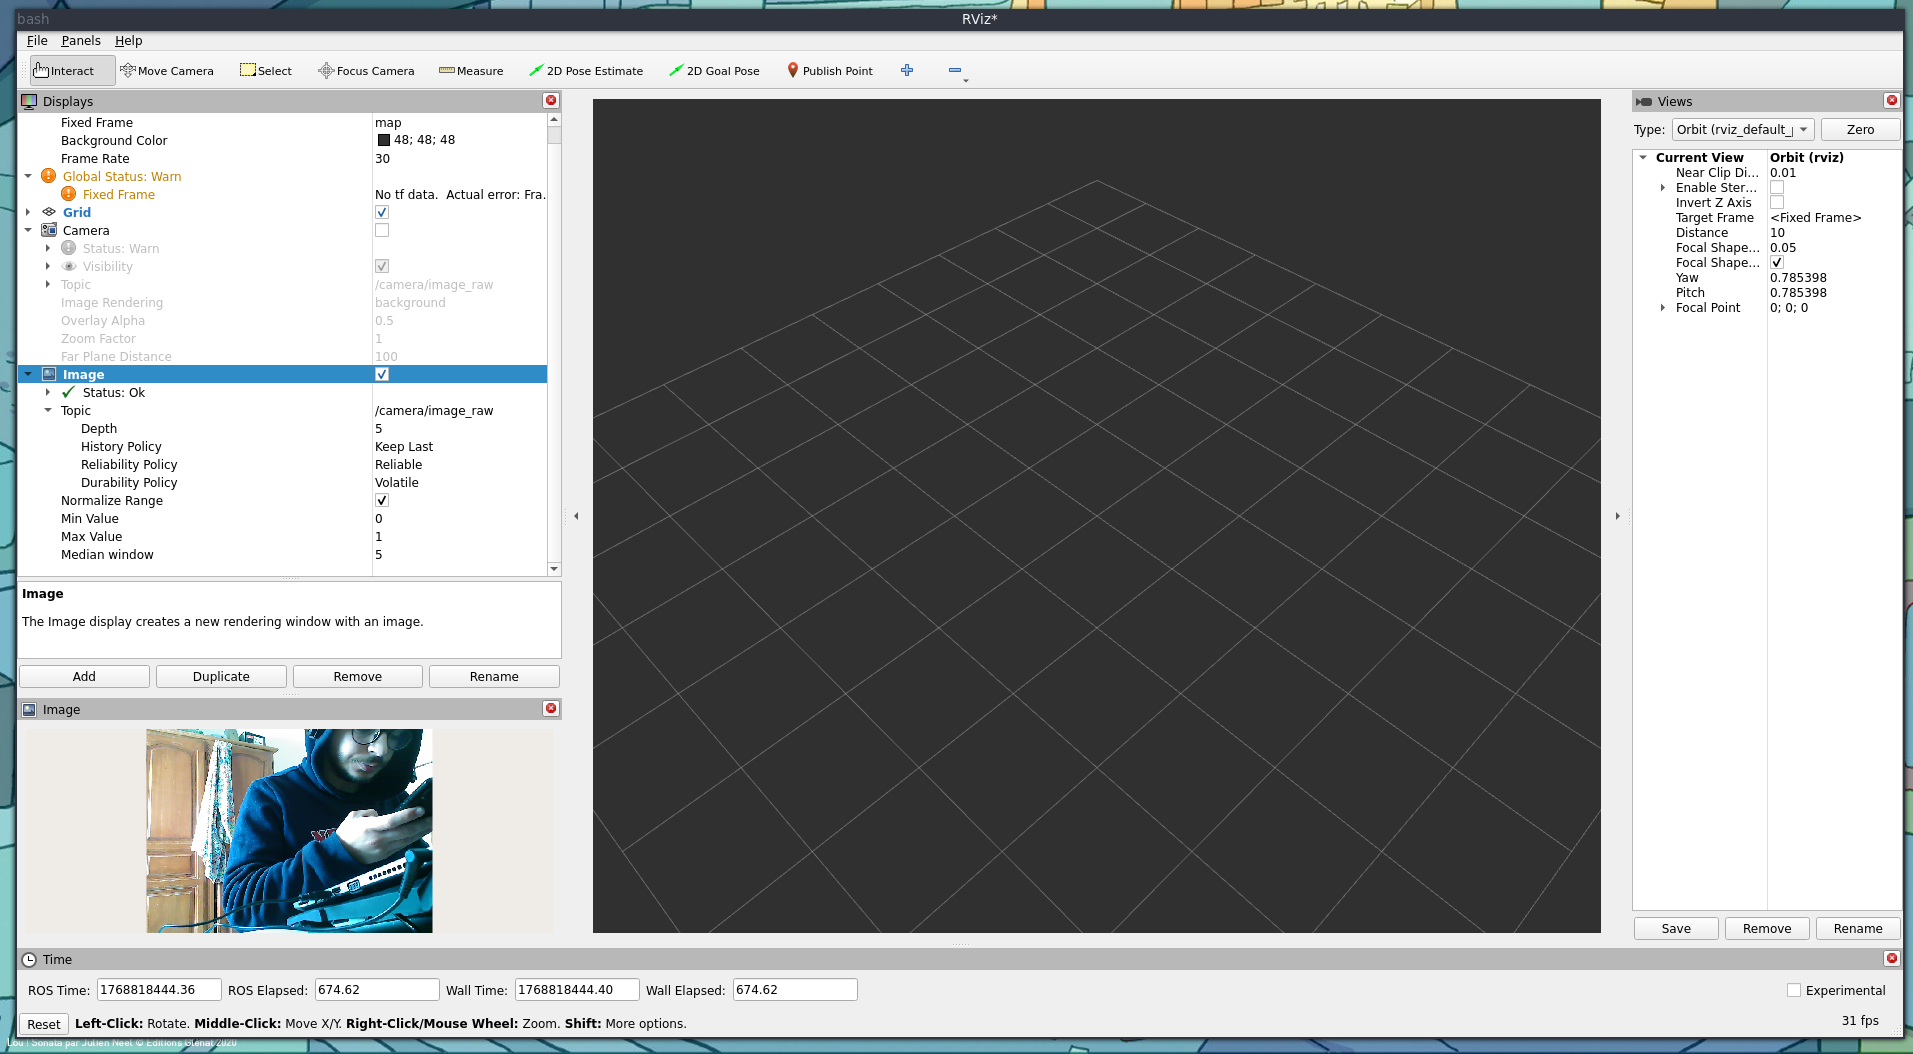
\includegraphics[width=\textwidth]{ros2_pic/2.png}
			\caption{RViz2 subscribing to \texttt{/camera/image\_raw} topic showing live camera feed}
			\label{fig:rviz_raw}
		\end{subfigure}
		\begin{subfigure}{0.45\textwidth}
			\centering
			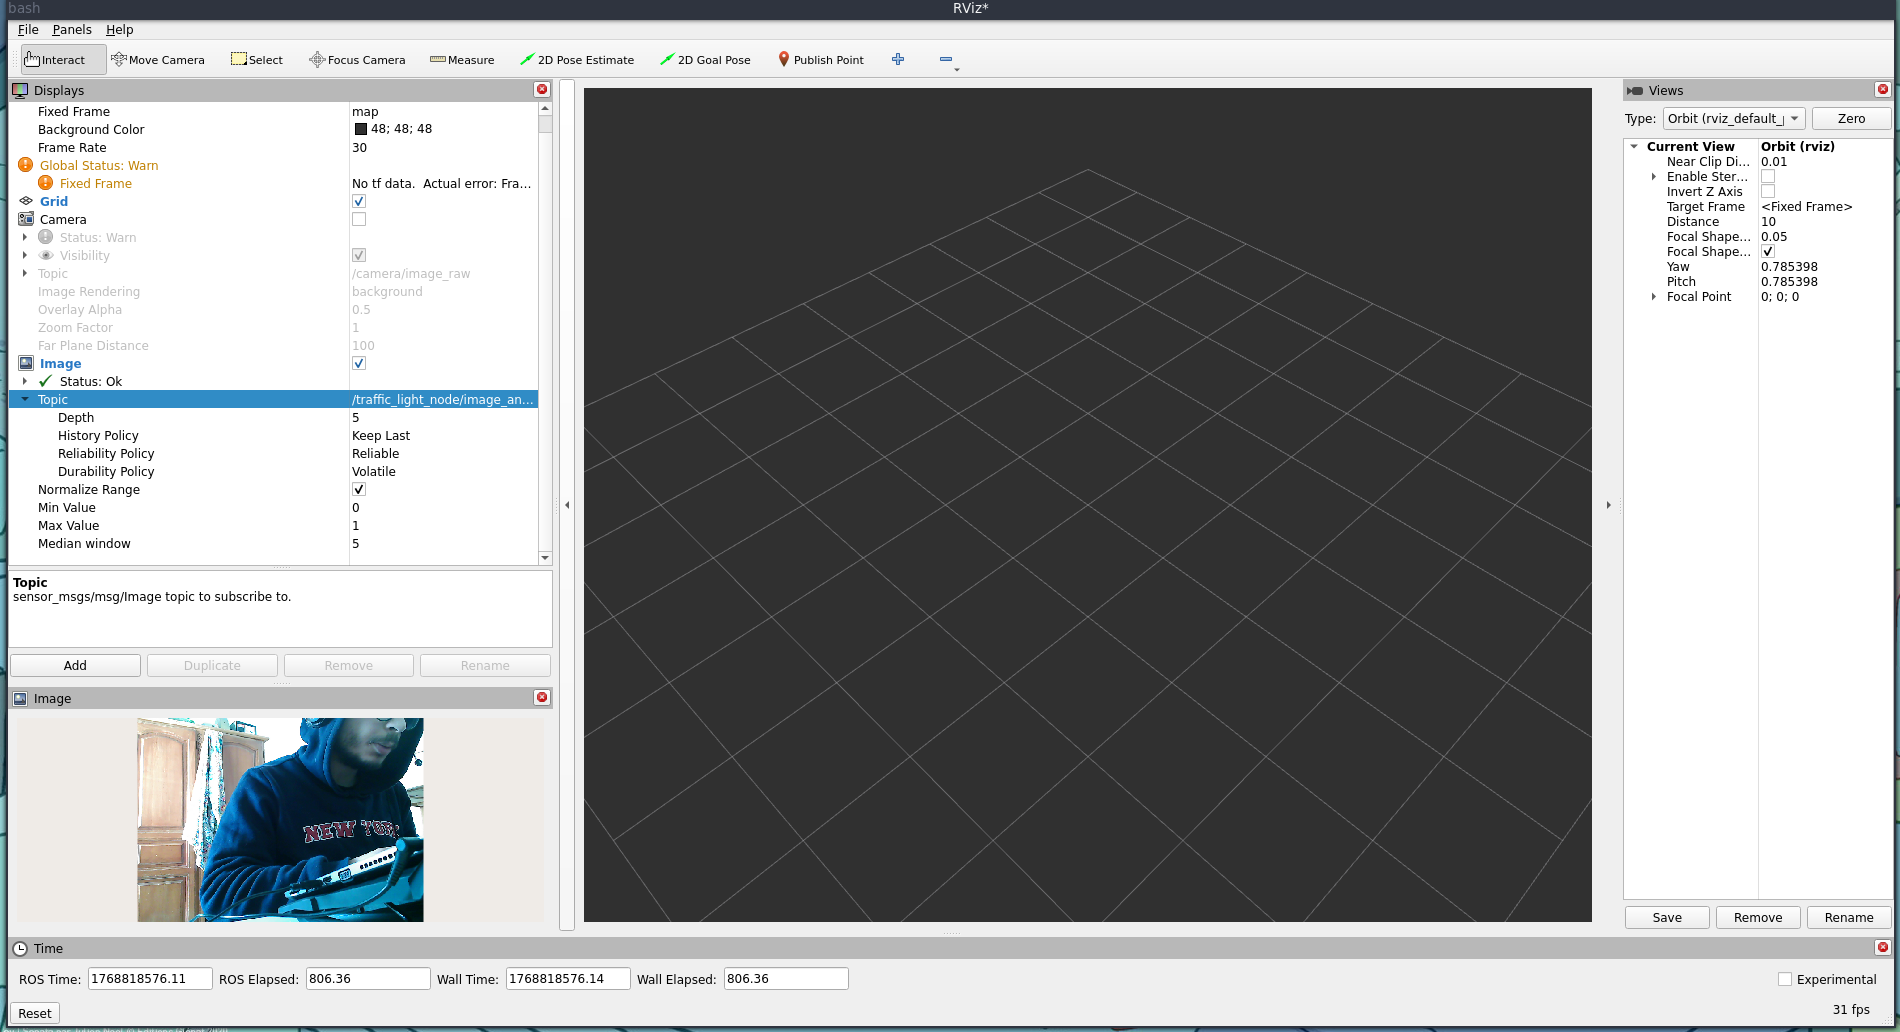
\includegraphics[width=\textwidth]{ros2_pic/3.png}
			\caption{RViz2 subscribing to \texttt{/traffic\_light/image\_annotated} topic with visualization settings}
			\label{fig:rviz_annotated}
		\end{subfigure}
		\caption{RViz2 remote visualization from laptop}
		\label{fig:rviz_visualization}
	\end{figure}
	
	Figures \ref{fig:rviz_raw} and \ref{fig:rviz_annotated} show the remote visualization capabilities:
	\begin{itemize}
		\item Real-time camera feed visualization via \texttt{/camera/image\_raw}
		\item Annotated detection visualization via \texttt{/traffic\_light/image\_annotated}
		\item Configurable display parameters in RViz2 interface
		\item Low-latency visualization over local WiFi network
	\end{itemize}
	
	\subsection{Traffic Light Detection Results}
	\begin{figure}[H]
		\centering
		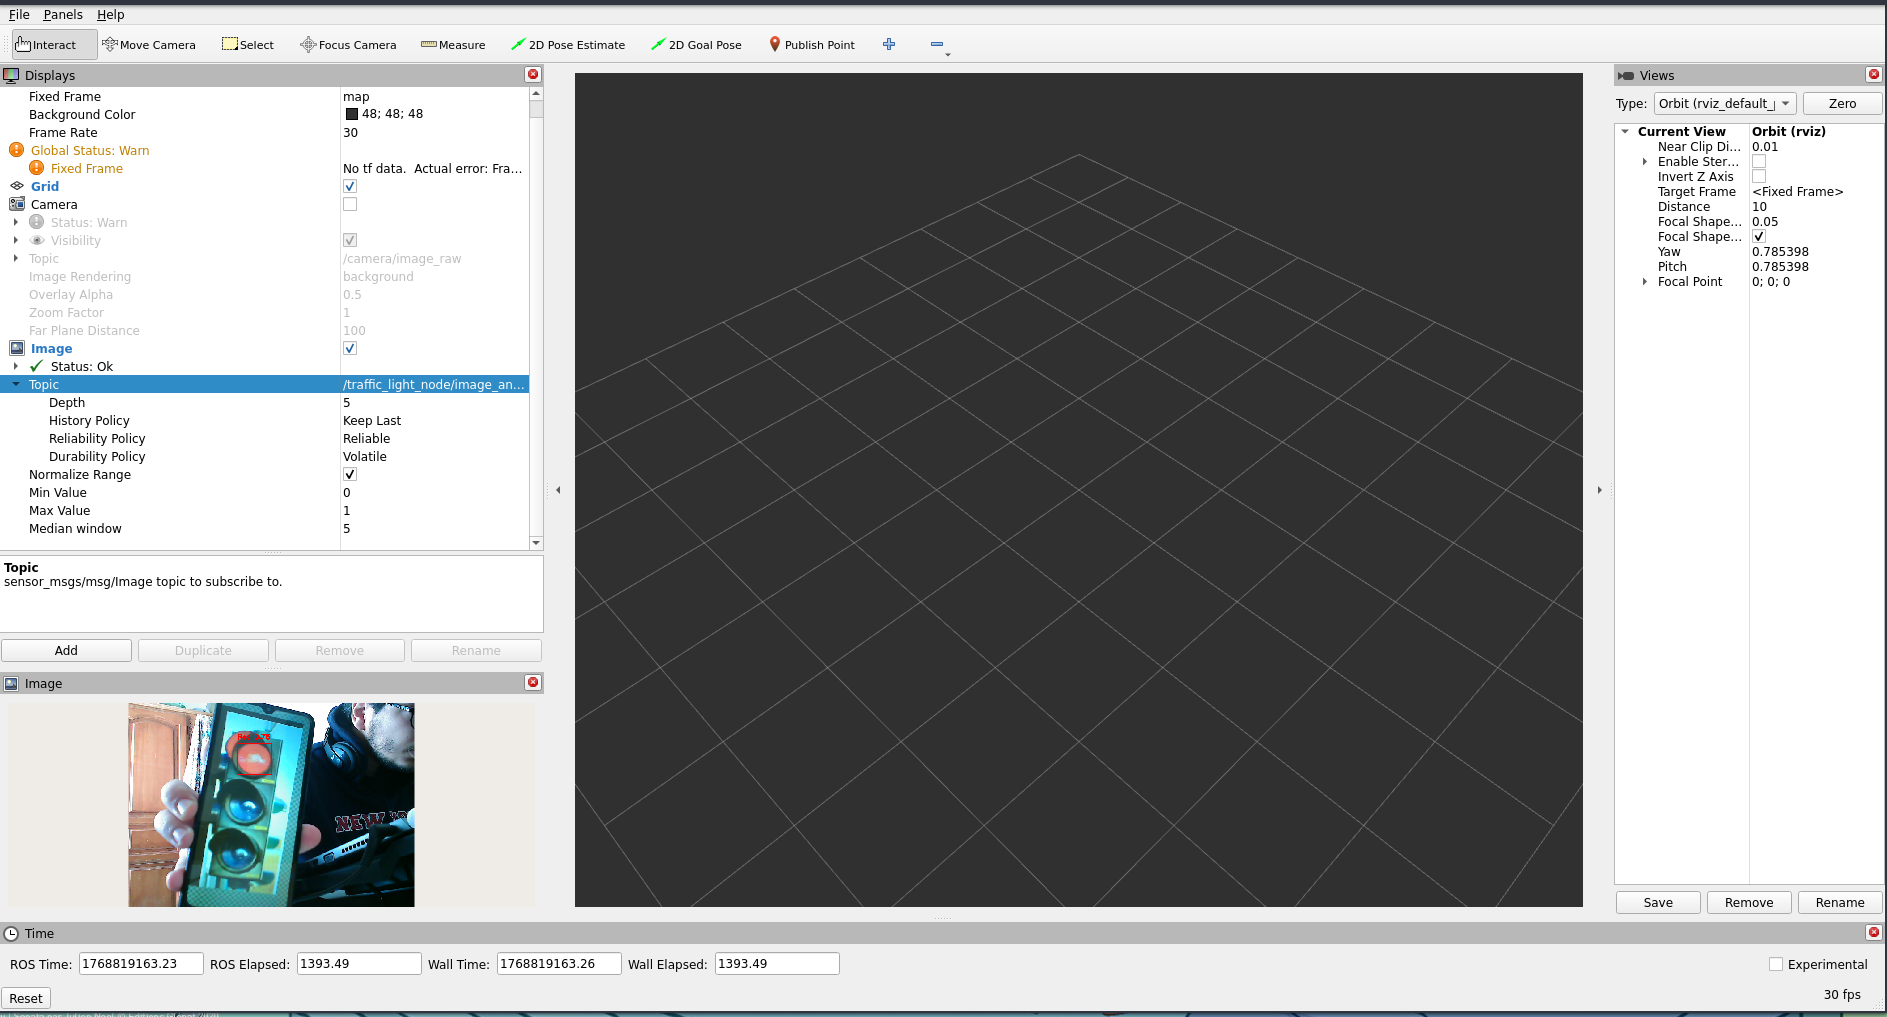
\includegraphics[width=0.8\textwidth]{ros2_pic/4.png}
		\caption{Successful red traffic light detection with bounding box annotation and topic configuration showing subscription to \texttt{/traffic\_light/image\_annotated}}
		\label{fig:detection_result}
	\end{figure}
	
	Figure \ref{fig:detection_result} demonstrates the successful detection capabilities:
	\begin{itemize}
		\item Red traffic light accurately detected with bounding box
		\item Annotation showing confidence score and class label
		\item ROS topic configuration for visualization
		\item Real-time detection at approximately 20 FPS on Raspberry Pi
	\end{itemize}
	
	\subsection{ROS2 Packages}
	\begin{table}[H]
		\centering
		\begin{tabularx}{\textwidth}{|l|X|}
			\hline
			\textbf{Package} & \textbf{Functionality} \\
			\hline
			camera\_capture & Publishes raw camera images from Raspberry Pi camera \\
			vision\_perception & Traffic light detection and annotation pipeline \\
			traffic\_light\_node & Main detection node using TensorFlow Lite \\
			\hline
		\end{tabularx}
		\caption{ROS2 Package Structure}
	\end{table}
	
	\subsubsection{Topics and Communication}
	\begin{itemize}
		\item \texttt{/camera/image\_raw}: Raw camera feed from Raspberry Pi camera module
		\item \texttt{/traffic\_light/node/image\_annotated}: Annotated detection images with bounding boxes
		\item \texttt{/traffic\_light/detections}: Detection data including class, confidence, and coordinates
		\item \texttt{/position\_cmd}: Position commands to STM32 via UART bridge
		\item \texttt{/angular\_cmd}: Angular commands to STM32 via UART bridge
	\end{itemize}
	
	\subsection{Docker Container Setup}
	\begin{itemize}
		\item Custom Docker image supporting ROS2 Humble with ARM64 architecture
		\item TensorFlow Lite runtime integration for model inference
		\item OpenCV for image processing and camera interface
		\item Complete ROS2 workspace with all dependencies containerized
		\item Network configuration for remote visualization via RViz2
	\end{itemize}
	
	\section{System Integration}
	
	\subsection{Visualization System}
	\begin{itemize}
		\item RViz2 for ROS2 visualization over local WiFi network
		\item Real-time camera feed display with configurable parameters
		\item Detection bounding box visualization with class labels
		\item System status monitoring including topic activity and frame rates
		\item Remote access from any device on the local network
	\end{itemize}
	
	\section{Challenges and Solutions}
	
	\subsection{The Bare-Metal Integration Oversight}
	Developing the STM32 firmware bare-metal was an oversight regarding the requirements of the ROS2 ecosystem. \texttt{micro-ROS} requires an RTOS and complex DMA configurations that are difficult to implement from scratch in bare-metal C. The solution involved creating a custom UART communication protocol between the STM32 and Raspberry Pi.
	
	\subsection{Real-Time and System Stability Performance}
	\begin{itemize}
		\item \textbf{Challenge}: Ensuring real-time PID control on bare-metal STM32
		\item \textbf{Solution}: Optimized interrupt handling, efficient algorithms, and velocity ramping system
	\end{itemize}
	
	\subsection{Model Deployment on Resource-Constrained Hardware}
	\begin{itemize}
		\item \textbf{Challenge}: Limited computational resources on Raspberry Pi for real-time inference
		\item \textbf{Solution}: Model quantization to TensorFlow Lite format, efficient memory usage, and optimized pipeline
	\end{itemize}
	
	\section{Conclusion}
	
	This project successfully demonstrates a complete autonomous system integrating:
	\begin{itemize}
		\item Bare-metal embedded programming on STM32 with sophisticated velocity ramping
		\item Advanced PID control with smooth motion profiles
		\item Custom-trained YOLOv8 model for traffic light detection with 72\% mAP accuracy
		\item Efficient deployment using TensorFlow Lite on embedded Raspberry Pi hardware
		\item ROS2-based system architecture with Docker containerization
		\item Remote visualization via RViz2 over local WiFi network
		\item Successful real-time detection of traffic lights with annotated visualization
	\end{itemize}
	
	The velocity ramping system proved crucial for stable operation, while the custom traffic light detection model achieved sufficient accuracy for reliable real-world performance. The Docker-based ROS2 deployment on Raspberry Pi enabled consistent development and deployment, while remote RViz2 visualization allowed for convenient system monitoring. The integration of these components creates a robust autonomous platform suitable for various navigation applications.
	
	\section{Repository Links}
	\begin{itemize}
		\item \textbf{Odometry and STM32 Code}: \url{https://github.com/Onizuka09/OdometryRobot}
		\item \textbf{ROS2 and AI Implementation}: \url{https://github.com/Onizuka09/DagDeg_autonomous}
		\item \textbf{Model Training Notebook}: \url{https://colab.research.google.com/drive/1lxwcOyEtk-aGk_w2Za_TbaYP-JJjzC9H}
	\end{itemize}
\end{document}